\documentclass[twocolumn]{article}

\usepackage[top=.5in, bottom=.5in, left=.75in, right=.75in]{geometry}
\usepackage{url}
%\usepackage{hyperref}
\usepackage{graphicx}

\title{Reverse Engineering}
\author{Amir Vspades \\ \url{vegaspades@gmail.com}
				\and
				Sasan Rocky \\ \url{s.rocky@farhost.net}}
\date{}

\begin{document}
\maketitle

\begin{abstract}
This study compares the Forward Engineering and Backward Engineering (also
known as Reverse Engineering). In addition, some tools related to such field
have been reviewed.
\end{abstract}

\section{Introduction}\indent

\textbf{Reverse Engineering}, also called \textit{Backward Engineering}, is the
process by which a man-made object is de-constructed to reveal its designs,
architecture, or to extract knowledge from the object \cite{WEBSITE:1}. Reverse
Engineering is applicable in the fields of
\textit{Software Re-Engineering}.\newline

\textbf{Software Re-Engineering} is the examination and alteration of a system
to reconstitute it in a new form. The principles of Re-Engineering when applied
to the software development process is called software re-engineering. It
affects positively at software cost, quality, service to the customer and speed
of delivery \cite{WEBSITE:2}. Figure \ref{fig:fig1} illustrates the procedure of
Software Re-Engineering.\newline

\begin{figure*}
	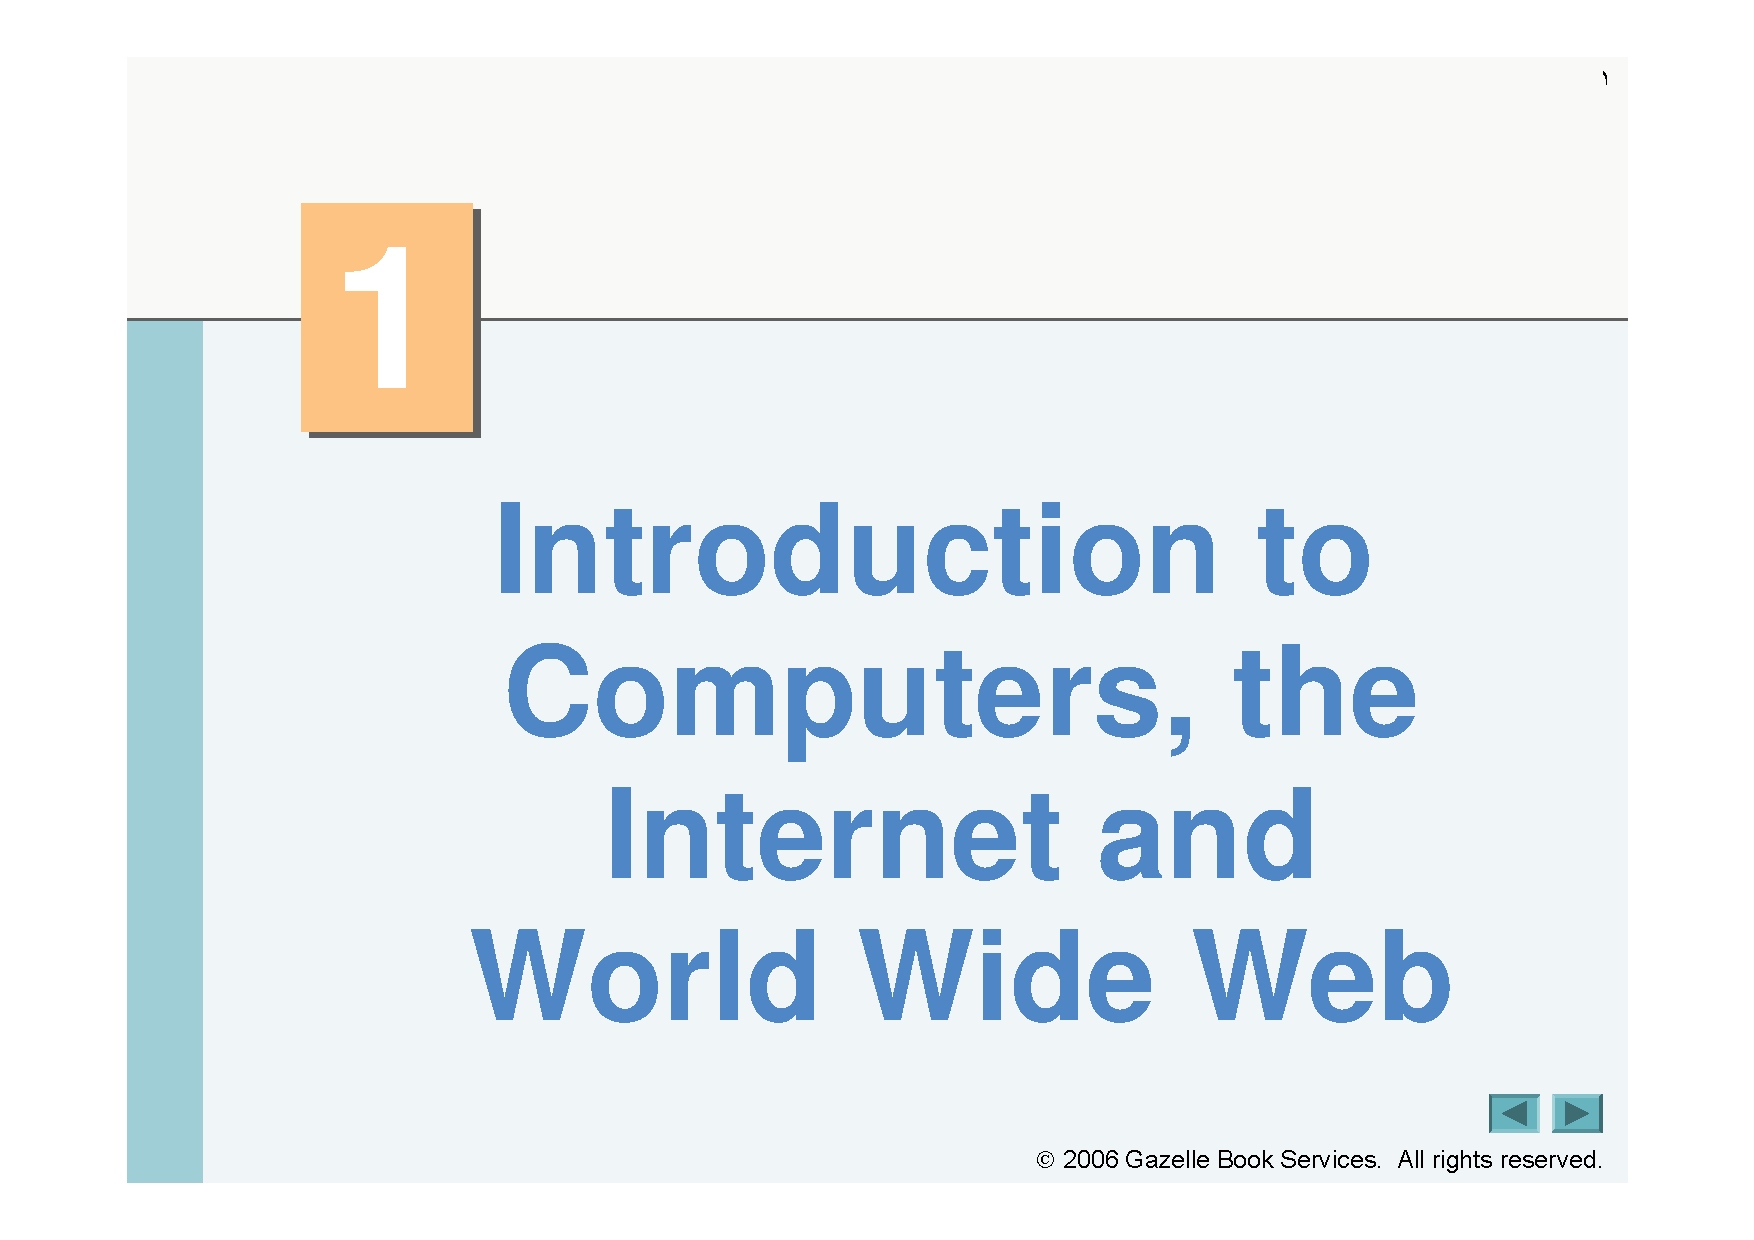
\includegraphics[width=\linewidth]{1.pdf}
	\caption{Forward Engineering vs. Backward Engineering}
	\label{fig:fig1}
\end{figure*}

\section{Reverse Engineering Tools}
All tools\footnote{Some of the tools mentioned in this article are archived and
accessible via this link: \url{http://mega.nz}}
that are useful in such field, could be categorized into the following
groups:
\begin{enumerate}
\item \textbf{Hex Editor}: A hex editor (or binary file editor or byte editor)
is a computer program that allows for manipulation of the fundamental binary
data that constitutes a computer file \cite{WEBSITE:3}.
\item \textbf{Debugger}: A debugger or debugging tool is a computer program used
to test and debug other programs (the ``target'' program) \cite{WEBSITE:4}.
\item \textbf{Disassembler}: A disassembler is a computer program that
translates machine language into assembly language \cite{WEBSITE:5}.
\item \textbf{Decompiler}: A decompiler is a computer program that takes an
executable file as input, and attempts to create a high level source file which
can be recompiled successfully \cite{WEBSITE:6}.
\item \textbf{Patcher}: A patch is a set of changes to a computer program or its
supporting data designed to update, fix, or improve it \cite{WEBSITE:7}. After
altering the $.EXE$ file, we could use a patcher to generate a new modified
$.EXE$ from the original one.
\item \textbf{Compressor}: A file archiver is a computer program that combines a
number of files together into one archive file, or a series of archive files,
for easier transportation or storage. File archivers may employ lossless data
compression in their archive formats to reduce the size of the archive
\cite{WEBSITE:8}.
\item \textbf{Analyzer}: Static program analysis is the analysis of computer
software that is performed without actually executing programs, in contrast with
dynamic analysis, which is analysis performed on programs while they are
executing \cite{WEBSITE:9}.
\item \textbf{Monitoring Tools} including:
	\begin{enumerate}
	\item Registry Monitor
	\item File Monitor
	\item Port Monitor
	\item Network Monitor
	\item Process Explorer
	\end{enumerate}
\item \textbf{Protector}: In software development, obfuscation is the deliberate
act of creating source or machine code that is difficult for humans to
understand \cite{WEBSITE:10}.
\end{enumerate}

\subsection{Hex Editor}
The following tools could be recognized as Hex Editors:
\begin{enumerate}
	\item Hiew \footnote{\url{http://www.hiew.ru/}}
	\item WinHex \footnote{\url{http://www.winhex.com/winhex/}}
	\item Hackman Suite \footnote{\url{https://www.technologismiki.com/prod.php?id=31}}
	\item Hex Workshop \footnote{\url{http://www.hexworkshop.com/}}
\end{enumerate}

\subsection{Debugger}
The following tools could be recognized as Debuggers:
\begin{enumerate}
	\item NuMega SoftICE \footnote{\url{https://archive.org/details/NuMega_SoftIce_Windows_3.2}}
	\item WinDbg \footnote{\url{https://docs.microsoft.com/en-us/windows-hardware/drivers/debugger/debugger-download-tools}}
	\item OllyDbg \footnote{\url{http://www.ollydbg.de/}}
	\item IDA Pro \footnote{\url{https://www.hex-rays.com/products/ida/}}
\end{enumerate}

\subsection{Disassembler}
The following tools could be recognized as Disassemblers:
\begin{enumerate}
	\item WinDasm \footnote{\url{https://vetusware.com/download/windasm\%208.93/?id=12732}}
	\item ilDasm \footnote{\url{https://docs.microsoft.com/en-us/dotnet/framework/tools/ildasm-exe-il-disassembler}}
\end{enumerate}

\subsection{Decompiler}
The following tools could be recognized as Decompilers:
\begin{enumerate}
	\item JAD \footnote{\url{https://web.archive.org/web/20080214075546/http://www.kpdus.com/jad.html}}
	\item Reflector \footnote{\url{https://www.red-gate.com/products/dotnet-development/reflector/}}
	\item SWF Decompiler \footnote{\url{https://www.sothink.com/product/flashdecompiler/}}
\end{enumerate}

\subsection{Patcher}
The following tools could be recognized as Patchers:
\begin{enumerate}
	\item Patch-Engine\footnote{\url{https://www.softpedia.com/get/Programming/Other-Programming-Files/Advanced-Patch-Engine.shtml}}
\end{enumerate}

\subsection{Compressor}
The following tools could be recognized as Compressors:
\begin{enumerate}
	\item UPX \footnote{\url{https://upx.github.io/}}
	\item ASPack \footnote{\url{http://www.aspack.com/}}
	\item PECompact \footnote{\url{https://bitsum.com/portfolio/pecompact/}}
\end{enumerate}

\subsection{Analyzer}
The following tools could be recognized as Analyzers:
\begin{enumerate}
	\item PEBrowse Professional \footnote{\url{https://download.cnet.com/PEBrowse-Professional-64-bit/3000-2218_4-75176627.html}}
\end{enumerate}

\subsection{Monitoring Tool}
The following tools could be recognized as Monitoring Tools:
\begin{enumerate}	
	\item RegMon \footnote{\url{https://docs.microsoft.com/en-us/sysinternals/downloads/regmon}}
	\item FileMon \footnote{\url{https://docs.microsoft.com/en-us/sysinternals/downloads/filemon}}
	\item ListDLLs \footnote{\url{https://docs.microsoft.com/en-us/sysinternals/downloads/listdlls}}
	\item PsList \footnote{\url{https://docs.microsoft.com/en-us/sysinternals/downloads/pslist}}
	\item TCPView \footnote{\url{https://docs.microsoft.com/en-us/sysinternals/downloads/tcpview}}
	\item WinObj \footnote{\url{https://docs.microsoft.com/en-us/sysinternals/downloads/winobj}}
\end{enumerate}

\subsection{Protector}
The following tools could be recognized as Monitoring Protectors:
\begin{enumerate}
	\item armadillo \footnote{\url{https://github.com/patrickfav/armadillo/blob/master/README.md}}
	\item obfuscator \footnote{\url{https://obfuscator.io/}}
\end{enumerate}

\section{Conclusion}
In this article, we reviewed the concept of Reverse Engineering along with a set
of tools regarding that title.

\bibliography{src}
\bibliographystyle{ieeetr}

\end{document}
